\section{Topologia} 
\definizione{}{
    Sia\marginnote{4 ott 2021} $ A \subseteq \R^{n} $, $ A $ si dice \textit{aperto} in $ \R^{n} $ se $ \forall\, x \in A $ $ \exists\, r>0 $ tale che $ B_r(x) \subseteq A $
}

\esempio{\label{es:gigio}\newcounter{estizio}\addtocounter{estizio}{\theesempi}
    $ R>0 $, sia \[D_{R}=\{x \in \R^{n}\,\tc\: |x| < R\} \] il disco di raggio $ R $. Dimostriamo che $ D_{R} $ è aperto.

    Dato $ x \in D_{R}  $, consideriamo $ r>0 $ tale che $ 0<r<R-|x| $ 
    
    $\implies$ $ r+|x|<R $.

    Verifichiamo che $ B_{r} \subseteq D_{R}$ ossia che $ \forall\, y \in B_{r}(x) $, $ |y|<R $ \[
        |y|=|y+x-x|\le \parentesi{<r}{|y-x|}+|x| \le r - |x| <R
       \] 
       
       $\implies$ $ B_{r}(x) \subseteq D_{R}$ 
       
       $\implies$ $ D_{R}  $ è aperto.

       $ D_{R}  $ si chiamerà \textit{disco aperto} di $ R $, ed è aperto e non limitato.
       \begin{center}
        In $ \R^{2} $

           \begin{tikzpicture}[scale=1.5, spy using outlines={circle, magnification=4, size=6cm, connect spies}]
            \fill [green!5] (0,0) circle (1.4);
               \draw [-stealth] (-2, 0) -- (3, 0);
               \draw [-stealth] (0, -2) -- (0, 2);
               \draw [dashed, green] (0,0) circle (1.4);
               \draw (1.11808971407,0.84254103241) -- (0,0);
               \fill (0.79863551004,0.60181502315) circle (0.03);
               \draw [dashed] (0.79863551004,0.60181502315) circle (0.3);
               \draw [dotted] (0.79863551004,0.60181502315) -- (0.55288989675, 0.77388795405);
               \node at (0.85, 0.45) {$x$};
               \draw [decorate, decoration = {calligraphic brace, raise = 2pt, amplitude = 4pt}] (0.04,0) -- (0.80263551004,0.60181502315);
                \node [rotate=37] at (0.235, 0.555) {$|x|$};
                \node at (1.3, 1) {$R$};
                \node at (0.5, 0.82) {$r$};
                \begin{scope}
                    \spy[red,size=6cm] on (1.2,0.9) in node [fill=white] at (4,1);
                \end{scope}
           \end{tikzpicture}
       \end{center}
}
\begin{minipage}{\textwidth}
\esempio{}{
    Sia $ E=\{z=(x,y) \in \R^{n}\,\tc\, y<x\} $
    \begin{center}
        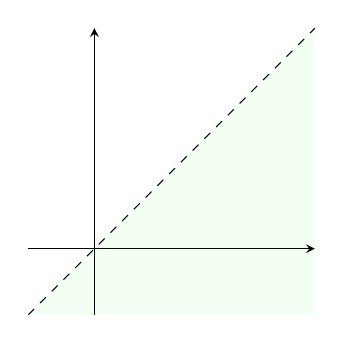
\begin{tikzpicture}[scale=1.4]
            \draw [color=black!0, fill=green!5] (-0.6, -0.6) -- (2, -0.6) -- (2,2) -- cycle;
            \draw [-stealth] (-0.6, 0) -- (2, 0);
            \draw [-stealth] (0,-0.6) -- (0,2);
            \draw [dashed] (-0.6, -0.6) -- (2,2);
        \end{tikzpicture}
    \end{center}

    $ z_0 \in E $, $ z_0=(x_0, y_0) $, $ y_0<x_0 $. Consideriamo la distanza di $ z_0 $ dalla retta $ s:y=x $, $ d(z_0, s) $ \[
        d(z_0, s) =\frac{|x_0-y_0|}{\sqrt{2}}
    \]
    
    Fissato $ 0<r<\frac{|x_0-y_0|}{\sqrt{2}}\displaystyle $ 
    
    $\implies$ $ B_{r}(z_0) \subseteq E  $. $ E $ è aperto e non limitato.
}
\end{minipage}
\esempio{}{
    Sia $ R>0 $, \[
        G_{R}=\{x \in \R^{n}; |x|\ge R\} 
    \] (vedasi Figura \ref{fig:1})
    \begin{figure}
    \begin{center}
        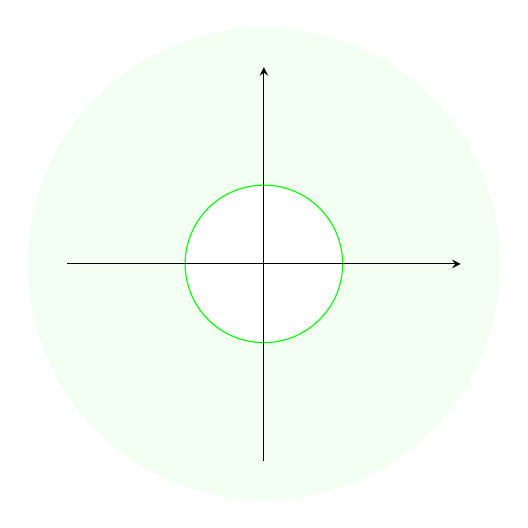
\begin{tikzpicture}
            \fill [green!5] (0,0) circle (3);
            \fill [white] (0,0) circle (1);
            \draw [green] (0,0) circle (1);
            \draw [-stealth] (-2.5, 0) -- (2.5, 0);
            \draw [-stealth] (0, -2.5) -- (0, 2.5);
        \end{tikzpicture}
    \end{center}
    \caption{$ G_{R}  $ in $ \R^{2} $}
    \label{fig:1}
    \end{figure}
    \begin{gather*}
        x_0=(R, 0, \cdots, 0)\\
        x_0 \in G_{R} \\
        \forall\, \varepsilon>0\quad \begin{aligned}
            x_1&=(R+ \varepsilon, 0, \cdots, 0) \subseteq G_{R}\\
            x_2&=(R- \varepsilon, 0, \cdots, 0) \nsubseteq  G_{R}
        \end{aligned}
    \end{gather*} 
    
    $\implies$ $ G_{R}  $ non è aperto.
}
\definizione{}{
    $ A \subseteq \R^{n} $ è \textit{chiuso} (in $ \R^{n} $) se l'insieme $ A^{C} $ è aperto: \[A^{C}= \R^{n}\setminus A = \{x \in \R^{n}; x \notin A\}.
    \]
}
\esempio{}{
    Dato $G_{R}=\{x \in \R^{n}; |x|\ge R\} $, \[D_{R}=G_{R}^{C}=\{x \in \R^{n}, |x|<R \} \] è aperto (vedasi esempio \hyperref[es:gigio]{\thesection.\theestizio}) 
    
    $\implies$ $ G_{R}  $ è chiuso.
}
\esempio{}{
    Sia \begin{align*}
        \overline{D_{R}}&=\{x \in \R^{n}, \, |x|\le R\}\\
        \overline{D_{R}^{C}}=\R^{n}\setminus \overline{D_{R}}& =\{x \in \R^{n},\,|x|>R\}
    \end{align*}

    Sia $ 0<r<|x|-R $. Consideriamo $ z \in B_{r}(x)  $
    \begin{equation*}
        |z|=|z-x+x|=|x-(x-z)|
        \ge \big||x|-\parentesi{<r}{|x-z|}\big|\ge |x|-r>R
    \end{equation*} 

    $\implies$ $ \forall\, z \in B_{r}(x)$, $ |z|>R $ 
    
    $\implies$ $ B_{r}(x) \subseteq \overline{D_{R}^{C} }  $ 
    
    $\implies$ $ \overline{D_{R}^{C} } $ è aperta 
    
    $\implies$ $ \overline{D_{R} } $ è chiuso.
}
\esempio{}{
    Dati $ 0<r<R $, è definita corona circolare l'insieme:
    \[
        C_{R,r}=\big\{z=(x,y) \in \R^{2}; r^{2}<x^{2}+y^{2}\le R^{2}\big\} 
    \]
    \begin{center}
        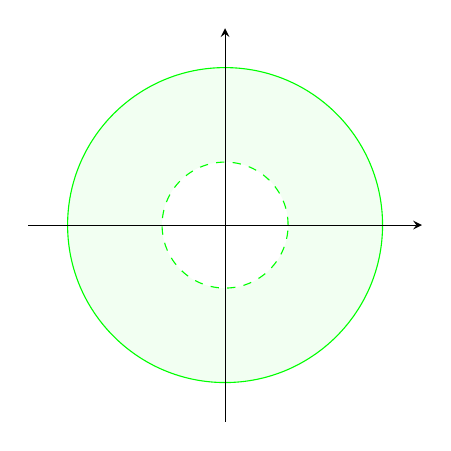
\begin{tikzpicture}
            \fill [green!5] (0,0) circle (2);
            \fill [white] (0,0) circle (0.8);
            \draw [green] (0,0) circle (2);
            \draw [dashed, green] (0,0) circle (0.8);
            \draw [-stealth] (-2.5, 0) -- (2.5, 0);
            \draw [-stealth] (0, -2.5) -- (0, 2.5);
        \end{tikzpicture}
    \end{center}
    $ C_{R, r}  $ non è aperto, \[
        C_{R,r}^{C}=\big\{z=(x,y) \in \R^{2}, x^{2}+y^{2}\le r^{2}\,\lor\, x^{2}+y^{2}> R^{2}\big\} 
    \] 
    
    $\implies$ $ C_{R,r}^{C} $ non è aperto.

    Concludiamo che $ C_{R,r}  $ non è né aperto né chiuso.
}  
\paragraph{Domanda}\begin{itemize}
    \item $ \emptyset $ è aperto? \[
        x \in \emptyset \,\implies\, \exists\, r>0\,\tc\, B_{r}(x) \subseteq \emptyset 
    \] 
    
    $\implies$ è sempre vera perché $ x \in \emptyset $ è falsa. 
    
    $\implies$ $ \emptyset $ è aperto.
    \item $ \R^{n} $ è aperto? $ \forall\,x \in \R^{n} $, $ \exists\, r>0 $ tale che $ B_{r}(x) \subseteq \R^{n}  $.
    \item $ \R^{n}=\R^{n}\setminus \emptyset $ 
    
    $\implies$ $ \R^{n} $ è complementare di un insieme aperto, ovvero è chiuso.
    \item $ \emptyset = \R^{n}\setminus \R^{n} $ 
    
    $\implies$ $ \emptyset $ è complementare di un insieme aperto, ovvero è chiuso.
    \item $ \emptyset $ e $ \R^{n} $ sono sia aperti che chiusi: sono gli unici due.
\end{itemize}
\definizione{}{
    Sia $ E \subseteq \R^{n} $ \begin{itemize}
        \item $ x_0 \in E $, diciamo che $ x_0 $ è \textit{interno} ad $ E $ se $ \exists\, r>0 $ tale che $ B_{r}(x_0) \subseteq E $;
        \item $ x_1 \in \R^{n} $, diciamo che $ x_1 $ è \textit{esterno} ad $ E $ se $ x_1 $ è interno a $ E^{C}=\R^{n}\setminus E $ 
        
        $\implies$ $ \exists\, r_1>0 $ tale che $ B_{r_1}(x_1) \subseteq E^{C}  $
        \item $ x_2 \in \R^{n} $, diciamo che $ x_2 $ è \textit{di frontiera} per $ E $ se $ x_2 $ non è interno ad $ E $ e $ x_2 $ non è esterno ad $ E $.
    \end{itemize}
} 
\notazione{}{
    $\mathring{E}$ è l'insieme di tutti i punti interni di $ E $: \begin{itemize}
        \item $ x_0 $ interno $\implies$ $ x_0 \in \mathring{E}$;
        \item $ x_0 $ esterno $\implies$ $ x_0 \in \mathring{E}^{C}$;
        \item $ x_0 $ di frontiera $\implies$ $ x_0 \notin\mathring{E} \,\land\, x_0\notin\mathring{E}^{C}$ 
        
        $\implies$ $ x_0 \in \partial E $
    \end{itemize}
}
\osservazione{}{
    \begin{itemize}
        \item $ \partial E =\partial E^{C} $;
        \item $ x_0 \in \mathring{E}$ $\implies$ $ x_0 \in E $ $\implies$ $ \mathring{E} \subseteq E $;
        \item $ x_0 \in \partial E $ non abbiamo informazioni sull'appartenenza di $ x_0 $ ad $ E $.
    \end{itemize}
}
\proprieta[(di caratterizzazione degli aperti)]{
    Dato $ A \subseteq \R^{n} $, 
    
    $ A $ è aperto $ \iff $ $ A=\mathring{A} $.
}
\begin{proof} Dimostriamo le due implicazioni:

    \begin{itemize}
        \item [``$\impliedby$''] $ \forall\,x \in A $ $\implies$ $ x \in \mathring{A}$ 
        
        $\implies$ $ \exists\, r>0$ tale che $ B_{r}(x) \subseteq A$ 
        
        $\implies$ $ A $ è aperto.
        \item [``$\implies$''] Assumiamo $ A $ aperto; $ \mathring{A} \subseteq A $ sempre.
        
        $ \forall\, x \in A $, $ \exists r >0 $ tale che $ B_{r}(x) \subseteq A$ 
        
        $\implies$ $x$ è interno 
        
        $\implies$ $ A \subseteq \mathring{A} $\qedhere
    \end{itemize}
\end{proof}

\teorema[(di caratterizzazione dei chiusi)]{carchiusdijooijooijdjkdjjdjdjdj}{
    Dato $ E \subseteq \R^{n} $, le seguenti proprietà sono equivalenti
    \begin{itemize}
        \item [(\textit{i})] $ E $ è chiuso;
        \item [(\textit{ii})] $ \partial E \subseteq E$;
        \item [(\textit{iii})] $ E' \subseteq E $, dove con $ E' $ indichiamo tutti i punti di accumulazione di $ E $.
    \end{itemize}
}
\dimostrazione{carchiusdijooijooijdjkdjjdjdjdj}{
    \begin{itemize}
        \item [(\textit{i}) $ \implies $ (\textit{ii})] $ E $ chiuso $ \implies $ $ \partial E \subseteq E $
        
        $ \forall\,x \in \partial E $, $ x\notin \mathring{E}^{C} $, ma $ \mathring{E}^{C} $ è aperto 
        
        $\implies$ $ \mathring{E}=\mathring{E}^{C} $ 
        
        $\implies$ $ x \in E $ 
        
        $\implies$ $ \partial E \subseteq E $
        \item [(\textit{ii}) $ \implies $ (\textit{iii})] $ \partial E \subseteq E$ $ \implies $ $ E' \subseteq E $
        
        \[
            \forall\, x \in E', \forall\, r >0\: \exists\, y \neq x \in E, y \in B_{r}(x) 
        \]
        osserviamo che $ x \in E' $ $\implies$ $ x \notin \mathring{E^{{C}}} $, infatti se per assurdo $ x \in \mathring{E^{{C}}} $ \[
            \exists\, r>0\,\tc\: B_{r}(x) \subseteq E^{C} \,\implies\, B_{r}(x)\cap E = \emptyset  
        \] 
        
        $\implies$ $ x \notin E' $
        \begin{itemize}
            \item caso \textit{a}: $ x \in \partial E $, visto che $ \partial E \subseteq E $ 
            
            $\implies$ se $ x \in E' $, allora $ x \in E $
            \item caso \textit{b}: $ x \in \mathring{E} $ $ \implies $ $ x \in E $
            
            Se $ x \in E' $, allora $ x \in E $
        \end{itemize}
        Ne risulta che $ E' \subseteq E $
        \item [(\textit{iii}) $ \implies $ (\textit{i})]
        %%%%%%%%%
    \end{itemize}
}